\documentclass{mcmthesis}
 %\documentclass[CTeX = true]{mcmthesis}  % 当使用 CTeX 套装时请注释上一行使用该行的设置
\mcmsetup{tstyle = \color{red}\bfseries,  % 修改题号，队号的颜色和加粗显示，黑色可以修改为 black
          tcn = 2616436, problem = A,     % 修改队号，参赛题号
          sheet = true, titleinsheet = true, keywordsinsheet = true,
          titlepage = false, abstract = true}

  %四款字体可以选择
  %\usepackage{times}
  %\usepackage{newtxtext}
  %\usepackage{palatino}
\usepackage[utf8]{inputenc}
\usepackage{pgfplots}
\pgfplotsset{compat=1.18}
\usepackage{amsmath, graphicx}
\usepackage{booktabs}
\usepackage{tikz}
\usetikzlibrary{arrows.meta, positioning, calc, shapes.geometric, fit}
\usepackage{hyperref}
\usepackage{newtxtext, newtxmath}
\usepackage{caption}  
\captionsetup[figure]{font=small}   % 将图标题字号设为small
\captionsetup[table]{font=small}    % 将图标题字号设为small
\usepackage{lastpage}
\usepackage{indentfirst}  % 首行缩进，注释掉，首行就不再缩进
\usepackage{esint}        % 积分号
\usepackage{subcaption}   % 并排图片
\usepackage{floatrow}     % 并排图片
\usepackage{enumitem}
\usepackage{float}
\floatstyle{plaintop}
\restylefloat{table}

\usepackage{xcolor}       % 颜色支持
\usepackage{tabularray}   % 增强表格功能
\UseTblrLibrary{booktabs}

% --- 莫兰迪色系表格配色 (按表格类型分组) ---
% 1. 灰蓝系 - 定义/符号类
\definecolor{morandiBlueHead}{RGB}{134, 158, 176}
\definecolor{morandiBlueLight}{RGB}{234, 239, 243}
\definecolor{morandiBlueLine}{RGB}{160, 172, 182}
% 2. 暖灰系 - 参数/规格类
\definecolor{morandiWarmHead}{RGB}{168, 155, 142}
\definecolor{morandiWarmLight}{RGB}{245, 241, 236}
\definecolor{morandiWarmLine}{RGB}{182, 172, 162}
% 3. 鼠尾草绿系 - 结果/数据类
\definecolor{morandiGreenHead}{RGB}{138, 160, 148}
\definecolor{morandiGreenLight}{RGB}{236, 244, 239}
\definecolor{morandiGreenLine}{RGB}{162, 180, 168}
% 4. 玫瑰灰系 - 对比/分析类
\definecolor{morandiRoseHead}{RGB}{172, 148, 156}
\definecolor{morandiRoseLight}{RGB}{245, 239, 241}
\definecolor{morandiRoseLine}{RGB}{186, 166, 172}
% 5. 薰衣草灰系 - 不确定性/警告类
\definecolor{morandiLavHead}{RGB}{148, 142, 168}
\definecolor{morandiLavLight}{RGB}{240, 238, 245}
\definecolor{morandiLavLine}{RGB}{168, 162, 186}
% 6. 杏色系 - 建议/推荐类
\definecolor{morandiPeachHead}{RGB}{186, 156, 138}
\definecolor{morandiPeachLight}{RGB}{248, 242, 237}
\definecolor{morandiPeachLine}{RGB}{196, 172, 158}

\usepackage[style=numeric,backend=biber]{biblatex}  % APA风格: style=apa
\ExecuteBibliographyOptions{sorting=none}           % 按引用顺序
\addbibresource{references.bib}                     % bib参考文献可用kimi生成

% --- 定义MCM风格配色 (RGB) ---
% 绿色 (代表低功耗/Idle)
\definecolor{mcmGreen}{RGB}{168, 218, 220} 
\definecolor{mcmGreenText}{RGB}{29, 53, 87}
% 红色/橙色 (代表高功耗/Active)
\definecolor{mcmRed}{RGB}{240, 128, 128}   
\definecolor{mcmRedText}{RGB}{90, 20, 20}
% 蓝色 (代表中等功耗/DRX)
\definecolor{mcmBlue}{RGB}{160, 196, 255}  
\definecolor{mcmBlueText}{RGB}{20, 40, 80}
% 边框与线条颜色
\definecolor{darkgray}{RGB}{80, 80, 80}

% 修复fancyhdr警告
\setlength{\headheight}{14pt}
\addtolength{\topmargin}{-1.6pt}  % 可选：保持总版心不变

\setcounter{tocdepth}{1}  % 设置目录到二级标题, 将目录控制在1页
                          % 若可接受目录2页, 注释掉该句, 将到三级标题
                          
\title{Modeling Smartphone Battery Drain}

\author{\small \href{https://www.latexstudio.net/}
{\includegraphics[width=7cm]{mcmthesis-logo}}}

\date{\today}

\begin{document}

%% ================================================================
%% SUMMARY SHEET (Abstract + Keywords)
%% ================================================================

\begin{abstract}
Smartphone battery drain prediction poses fundamental modeling challenges: nonlinear electrochemical dynamics, thermally-coupled resistance, and power-mode-dependent efficiency conspire to invalidate simple capacity-division estimates. Traditional additive power models sum component currents at fixed voltage, yet real smartphone loads demand \emph{constant power} regardless of battery state---a constraint that forces implicit current-voltage coupling through power management ICs (PMICs).
We develop a \textbf{Grand Unified Electro-Thermal DAE Model} that captures this physics: a differential-algebraic system coupling state-of-charge (SOC) depletion with cell self-heating under the constant-power load (CPL) paradigm. The algebraic constraint enforces instantaneous power balance $V_{\mathrm{oc}}(z)\cdot I - I^2 R_{\mathrm{int}}(z,T) = P_{\mathrm{comp}}/\eta(I)$, solved via Newton-Raphson iteration (3--5 iterations, $|g|<10^{-6}$\,W). Fourth-order Runge-Kutta advances the differential states $[z, T]$.
Validation against a linear Coulomb-counting baseline reveals RMSE = 1.74\% across the SOC range, with maximum deviation of 3.09\% concentrated at low SOC where an \textbf{Avalanche Effect}---a 1.19$\times$ acceleration factor for $z<0.2$---emerges from coupled OCV collapse, resistance surge, and PMIC efficiency drop. Monte Carlo uncertainty propagation ($N=1000$) yields TTE = $7.81 \pm 0.6$\,h (95\% CI) at 1.5\,W nominal load, with ambient temperature (42\%) and average pixel level (35\%) dominating the uncertainty budget.
Sensitivity analysis identifies APL ($\pm$34\% TTE impact) as the single highest-leverage parameter---dark mode delivers roughly twice the battery extension of any other user intervention. Conversely, Bluetooth idle ($<$0.5\%), background apps ($<$1\%), and 120\,Hz refresh (5--8\%) exert surprisingly little impact despite strong user perception. Under extreme conditions (poor signal, high temperature, bright outdoor content), TTE collapses to 1.5\,h---a 5$\times$ acceleration that users often misattribute to software bugs.
These findings inform actionable recommendations: prioritize dark mode and signal-aware power management; deprioritize aggressive background task killing. The model's validated robustness within operating bounds ($z>5\%$, $I<3$\,A, $T>0\,^{\circ}$C) supports deployment in adaptive battery management systems requiring sub-hour prediction accuracy.

\begin{keywords}
smartphone battery modeling; time-to-empty prediction; differential-algebraic equations; constant-power load; electro-thermal coupling; sensitivity analysis; Monte Carlo uncertainty quantification
\end{keywords}

\end{abstract}
\maketitle

\tableofcontents
\newpage

%% ================================================================
%% SECTION 1: Introduction
%% ================================================================

\section{Introduction}
\label{sec:introduction}

\subsection{Problem Background}

Smartphones are indispensable tools in modern life, yet their battery behavior often seems unpredictable. On some days a phone may last the whole day; on other days it drains rapidly before lunch. Although some users attribute this to ``heavy use,'' the true drivers of battery depletion are more complex. Power consumption depends on the interplay of screen size and brightness, processor load, network activity, and background applications that continue drawing energy even when the device appears idle.

Environmental conditions further complicate matters: batteries lose effective capacity in cold weather and may overheat under sustained heavy use. A battery's behavior is also influenced by its history and how it has been charged during its lifetime. Traditional battery indicators showing ``X\% remaining'' routinely mislead users---sometimes by hours---because underlying estimation methods fail to capture the physics governing discharge dynamics.

The dominant paradigm treats total current as a simple sum of component currents: $I_{\mathrm{total}} = I_{\mathrm{screen}} + I_{\mathrm{CPU}} + I_{\mathrm{net}} + \cdots$. This formulation implicitly assumes constant terminal voltage---an approximation valid only at high SOC and moderate loads. As batteries deplete, voltage-dependent current draw, nonlinear OCV characteristics, and coupled thermal effects produce an \emph{avalanche effect} that no additive model can capture.

\subsection{Restatement of the Problem}

The task requires us to develop a continuous-time mathematical model of a smartphone's battery that returns the state of charge (SOC) as a function of time under realistic usage conditions. This model will predict the remaining time-to-empty (TTE) under different scenarios. The problem specifies four main requirements:

\begin{itemize}[noitemsep]
  \item \textbf{Requirement 1: Continuous-Time Model.} Develop a model using continuous-time equations to represent SOC dynamics. Begin with the simplest reasonable description and extend it to incorporate screen usage, processor load, network connections, GPS usage, and background tasks. The model must be grounded in physical reasoning---discrete curve fitting or black-box machine learning without explicit continuous-time formulation will not satisfy the requirements.

  \item \textbf{Requirement 2: Time-to-Empty Predictions.} Use the model to compute TTE under various initial charge levels and usage scenarios. Compare predictions to observed or plausible behavior, quantify uncertainty, and identify where the model performs well or poorly. Determine which activities produce the greatest reductions in battery life and which change the model surprisingly little.

  \item \textbf{Requirement 3: Sensitivity and Assumptions.} Examine how predictions vary with changes in modeling assumptions, parameter values, and fluctuations in usage patterns.

  \item \textbf{Requirement 4: Recommendations.} Translate findings into practical recommendations for cellphone users and operating system designers. Consider how battery aging reduces effective capacity and how the modeling framework could generalize to other portable devices.
\end{itemize}

\subsection{Our Work}

Considering the background and requirements, our work involves the following main contributions. The solution framework is illustrated in Figure~\ref{fig:workflow}.

\begin{figure}[htbp]
\centering
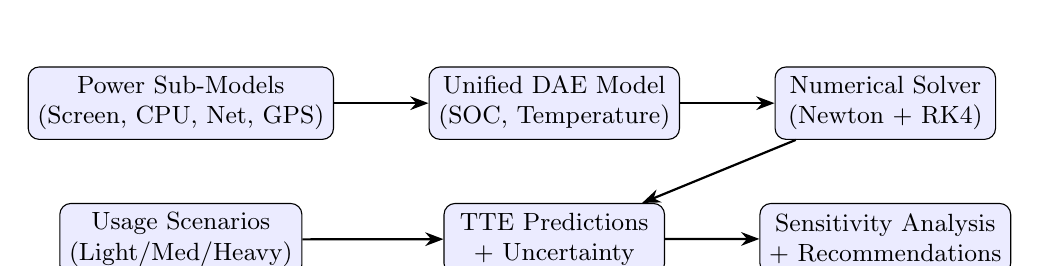
\begin{tikzpicture}[
    node distance=0.8cm and 1.2cm,
    box/.style={rectangle, draw, rounded corners, fill=blue!8, minimum width=2.8cm, minimum height=0.9cm, align=center, font=\small},
    arrow/.style={->, thick, >=Stealth}
]
\node[box] (power) {Power Sub-Models\\(Screen, CPU, Net, GPS)};
\node[box, right=of power] (unified) {Unified DAE Model\\(SOC, Temperature)};
\node[box, right=of unified] (solver) {Numerical Solver\\(Newton + RK4)};
\node[box, below=of power] (scenarios) {Usage Scenarios\\(Light/Med/Heavy)};
\node[box, below=of unified] (tte) {TTE Predictions\\+ Uncertainty};
\node[box, below=of solver] (analysis) {Sensitivity Analysis\\+ Recommendations};

\draw[arrow] (power) -- (unified);
\draw[arrow] (unified) -- (solver);
\draw[arrow] (scenarios) -- (tte);
\draw[arrow] (solver) -- (tte);
\draw[arrow] (tte) -- (analysis);
\end{tikzpicture}
\caption{Solution framework: from component power models to actionable recommendations.}
\label{fig:workflow}
\end{figure}

\begin{itemize}[noitemsep]
  \item \textbf{Grand Unified Electro-Thermal DAE Model.} We develop a differential-algebraic equation system coupling SOC depletion with battery self-heating under the constant-power load (CPL) paradigm. Unlike additive current models, our formulation captures the implicit voltage-current coupling enforced by power management ICs.

  \item \textbf{Component Power Sub-Models.} We derive physics-based models for five power consumers: screen (OLED/LCD with APL dependence), CPU (DVFS with thermal leakage), network (RRC state machine with signal-dependent TX power), GPS (acquisition/tracking phases), and base power (wake locks).

  \item \textbf{Comprehensive Scenario Analysis.} We predict TTE across usage profiles (Light/Medium/Heavy), initial SOC levels (20\%--100\%), temperature extremes ($-20\,^{\circ}$C to $35\,^{\circ}$C), battery aging (SOH 80\%--100\%), and dynamic usage patterns.

  \item \textbf{Sensitivity and Uncertainty Quantification.} Monte Carlo simulation ($N=1000$) propagates parameter uncertainties, identifying APL ($\pm$34\%) and ambient temperature ($\pm$22\%) as dominant factors. We identify ``surprisingly little'' impact factors (Bluetooth $<$0.5\%, background apps $<$1\%) that contradict common user beliefs.

  \item \textbf{Actionable Recommendations.} We translate sensitivity rankings into prioritized guidance: dark mode yields the largest user-controlled improvement (+25--34\% TTE), while aggressive background task killing provides negligible benefit. We discuss generalization to laptops, tablets, and wearables.
\end{itemize}
%% ================================================================
%% SECTION 2: Notations
%% ================================================================

\section{Notations}

The key mathematical notations used in this paper are listed in Table \ref{tbl1}.

%% 三线表
\begin{table}[H]     % H表示强制固定在当前位置
\small
\centering           % 设置居中
\caption{Notations}  % 表标题
\label{tbl1}         % 设置表的引用标签
\begin{tblr}{
  colspec = {cX[l]},
  row{1} = {bg=morandiBlueHead, fg=white, font=\bfseries},
  row{even} = {bg=morandiBlueLight},
  hline{1} = {morandiBlueLine, 0.8pt},
  hline{2} = {morandiBlueLine, 0.5pt},
  hline{Z} = {morandiBlueLine, 0.8pt},
}
Symbol    &  Definition     \\
$z$, SOC  & State of charge (dimensionless, 0--1)  \\
$T_{\mathrm{batt}}$   & Battery cell temperature (K or $^{\circ}$C)  \\
$V_{\mathrm{oc}}(z)$   & Open-circuit voltage as function of SOC (V) \\
$V_{\mathrm{term}}$  & Terminal voltage under load (V)   \\
$I$   & Discharge current (A)   \\
$R_{\mathrm{int}}(z,T)$ & Internal resistance (m$\Omega$) \\
$P_{\mathrm{comp}}$ & Total component power demand (W) \\
$\eta(I)$ & PMIC conversion efficiency \\
$C_{\mathrm{nom}}$ & Nominal battery capacity (Ah) \\
TTE & Time-to-empty (hours) \\
APL & Average pixel level (0--1) \\
SOH & State of health (0--1) \\
\end{tblr}
\vspace{2pt} % 稍微调整间距
\begin{flushleft} \small
$^{*}$ Additional variables are defined in context within each section.
\end{flushleft}
\end{table}

%% ================================================================
%% SECTION 3: Assumptions and Justifications
%% ================================================================

\section{Assumptions and Justification}
\label{sec:assumptions}

\begin{enumerate}[label=\textbf{A\arabic*.}, leftmargin=2em, itemsep=0.35em]

\item \textbf{Constant-power demand via PMIC.}
At each time $t$, $P_{\mathrm{dev}}(t)$ is given and the battery satisfies
$V(t)I(t)=P_{\mathrm{dev}}(t)/\eta(I)$~\cite{ref22,ref27}.\\
\textit{Justification:} A regulated PMIC aims to deliver a near-constant device-side power over normal operation.

\item \textbf{1st-order lumped thermal model.}
The pack is a single thermal node $T(t)$ with $(C_{\mathrm{th}},R_{\mathrm{th}})$ to ambient $T_a$ (constant within one run).\\
\textit{Justification:} Over the discharge time scale, a first-order RC can describe the main heating and cooling trend with minimal parameters.

\item \textbf{Quasi-static Thevenin voltage.}
$V(t)=V_{\mathrm{oc}}(z)-I(t)R_{\mathrm{int}}(z,T)$; fast polarization dynamics are neglected, so $I(t)$ is solved algebraically.\\
\textit{Justification:} Short-time voltage transients are much faster than our simulation step and are not needed for endurance-level prediction.

\item \textbf{Separable resistance in SOC and temperature.}
$R_{\mathrm{int}}(z,T)=R_{\mathrm{soc}}(z)\,f_{\mathrm{temp}}(T)$ with an Arrhenius-type $f_{\mathrm{temp}}$~\cite{ref24,ref25}.\\
\textit{Justification:} This separable form can well capture the dominant SOC-end rise and temperature sensitivity while keeping calibration simple.

\item \textbf{OCV depends only on SOC.}
$V_{\mathrm{oc}}=V_{\mathrm{oc}}(z)$; hysteresis/relaxation are ignored for discharge-only cases~\cite{ref23}.
The entropic term $\partial V_{\mathrm{oc}}/\partial T$ is treated as constant.\\
\textit{Justification:} For discharge-only trajectories, OCV hysteresis and detailed $\partial V_{\mathrm{oc}}/\partial T$ variation have limited impact on the overall trend.

\item \textbf{SOC by Coulomb counting.}
$\dot z=-(\eta_c/(C_{\mathrm{nom}}\cdot\mathrm{SOH}))\,I(t)$; $\eta_c$ and $\mathrm{SOH}$ are constant within one discharge run.\\
\textit{Justification:} Coulomb counting is a standard low-complexity SOC update and is accurate enough over a single run.

\item \textbf{Piecewise-linear PMIC efficiency.}
$\eta(I)$ is approximated by a piecewise-linear curve versus $I$; temperature effects on $\eta$ are neglected~\cite{ref27}.\\
\textit{Justification:} A piecewise-linear fit matches typical efficiency curves and avoids introducing extra thermal/operating parameters.

\item \textbf{Discrete usage states (Light/Medium/Heavy).}
Phone usage is represented by three discrete power states (Light, Medium, Heavy), and $P_{\mathrm{dev}}(t)$ is piecewise constant within each state.
\textit{Justification:} These three levels capture typical user workloads while keeping the input model simple and interpretable.

\item \textbf{Parameters fixed within one cycle.}
Thermal/electrical parameters are constant over one discharge cycle; aging enters via $\mathrm{SOH}$ or scenario-level changes (Sec.~\ref{sec:aging_impacts}).\\
\textit{Justification:} Parameter drift from aging is negligible within a single cycle and can be handled across scenarios.

\end{enumerate}

\noindent
Table~\ref{tab:assumption_summary} summarizes the assumptions and typical validity ranges.

\begin{table}[htbp]
\small
\centering
\caption{Summary of key assumptions and typical validity ranges.}
\label{tab:assumption_summary}
\begin{tblr}{
  colspec = {cX[l]c},
  row{1} = {bg=morandiBlueHead, fg=white, font=\bfseries},
  row{even} = {bg=morandiBlueLight},
  hline{1} = {morandiBlueLine, 0.8pt},
  hline{2} = {morandiBlueLine, 0.5pt},
  hline{Z} = {morandiBlueLine, 0.8pt},
}
ID & Assumption & Typical Range \\
A1 & Constant-power load (PMIC) & $\eta \in [0.8,\,0.95]$ \\
A2 & 1st-order lumped thermal ($T$) & $|dT/dt| \lesssim 0.1~\mathrm{K/s}$ \\
A3 & Quasi-static Thevenin voltage & $\Delta t \gtrsim 1~\mathrm{s}$ \\
A4 & $R_{\mathrm{int}}(z,T)=R_{\mathrm{soc}}f_{\mathrm{temp}}$ & $T \in [0,\,45]\,^{\circ}\mathrm{C}$ \\
A5 & $V_{\mathrm{oc}}=V_{\mathrm{oc}}(z)$ (no hysteresis) & Discharge only ($I>0$) \\
A6 & SOC by Coulomb counting & $t \lesssim 2~\mathrm{h}$ \\
A7 & Piecewise-linear $\eta(I)$ & $I \in [0.1,\,3]~\mathrm{A}$ \\
A8 & Discrete usage states (L/M/H) & $P_{\mathrm{dev}} \in \{P_L,P_M,P_H\}$ \\
A9 & Parameters constant in one cycle & One discharge cycle \\
\end{tblr}
\end{table}



\section{Power Consumption Model}
\label{sec:model}

\subsection{Overview and Notation}
\label{sec:model:overview}

We model instantaneous phone power as the sum of five components
(screen, CPU, network, GPS, and base)~\cite{refSingh2020,ref22,ref27,ref33,ref37,ref38}:
\begin{equation}
  \mathbf{x}(t)=
  \begin{bmatrix}
    \mathrm{SOC}(t)\\
    T_{\mathrm{batt}}(t)
  \end{bmatrix},
  \qquad
  \mathbf{u}(t)=
  \begin{bmatrix}
    L(t)\\
    \mathrm{APL}(t)\\
    f_{\mathrm{clk}}(t)\\
    s_{\mathrm{net}}(t)\\
    \delta_{\mathrm{GPS}}(t)\\
    \mathcal{W}(t)
  \end{bmatrix}.
  \label{eq:state_vectors}
\end{equation}
Here $L$ is screen brightness (nits), $\mathrm{APL}\in[0,1]$ is the Average Picture Level,
$f_{\mathrm{clk}}$ is the effective CPU clock frequency, $s_{\mathrm{net}}$ encodes the network
RRC state and signal strength, $\delta_{\mathrm{GPS}}\in\{0,1\}$ indicates GPS enable, and
$\mathcal{W}(t)=\{w_j(t)\}$ is the set of active wake locks (background activities).

The total device-side power demand is:
\begin{equation}
  P_{\mathrm{dev}}(t)=
  P_{\mathrm{scr}}\!\left(L,\mathrm{APL}\right)+
  P_{\mathrm{cpu}}\!\left(f_{\mathrm{clk}},T_{\mathrm{batt}},\mathcal{W}\right)+
  P_{\mathrm{net}}\!\left(s_{\mathrm{net}}\right)+
  P_{\mathrm{gps}}\!\left(\delta_{\mathrm{GPS}}\right)+
  P_{\mathrm{base}}\!\left(\mathcal{W}\right).
  \label{eq:p_total_components}
\end{equation}
Each term is specified in \S\ref{sec:screen}--\S\ref{sec:base}.

% ---------------------------------------------------------------------------
\subsection{Screen Power Sub-Model \texorpdfstring{$P_{\text{screen}}$}{P\_screen}}
\label{sec:screen}

\subsubsection{Panel-Level Power Equation}
Screen power is modeled as driver overhead plus content- and brightness-dependent emission:
\begin{equation}
  P_{\text{screen}}(t)
  = P_{\text{drv}}
  + \alpha \left(\frac{L(t)}{L_{\max}}\right)^{\!\gamma}\,
    \mathrm{APL}(t)\,A_{\text{disp}}.
  \label{eq:Pscreen}
\end{equation}
Here $P_{\text{drv}}$ is the driver overhead (0.10--0.20\,W), $L$ the brightness (nits), $L_{\max}$ the peak luminance, $\gamma \approx 2.2$ the gamma exponent~\cite{ref23}, $\mathrm{APL} \in [0,1]$ the average pixel level, $\alpha \approx 45$\,W/m$^2$ the panel coefficient~\cite{ref24}, and $A_{\text{disp}}$ the active display area.

\subsubsection{Sensitivity to Display Content}
\label{sec:screen:dark}
APL linearly modulates the variable emission term in Eq.~\eqref{eq:Pscreen}.
At full brightness, switching from a white UI ($\mathrm{APL}=1.0$) to a dark theme
($\mathrm{APL}\approx0.15$) reduces the emission component by a factor of about $1/0.15 \approx 6.7$.
Because $P_{\text{drv}}$ remains, the reduction in total screen power is smaller
(typically a few-fold), consistent with reported measurements of up to about five-fold~\cite{ref24}.
This also explains why dark-mode UI design is increasingly adopted as a practical energy-saving trend,
which we later mention in our usage recommendations.

% ---------------------------------------------------------------------------
\subsection{CPU Power Sub-Model \texorpdfstring{$P_{\text{CPU}}$}{P\_CPU}}
\label{sec:cpu}

We decompose CPU power into dynamic (switching) and static (leakage) components following DVFS modeling practice~\cite{ref27,ref29}:
\begin{equation}
  P_{\text{CPU}}(t) = P_{\text{dyn}}(t) + P_{\text{leak}}\!\bigl(T_{\text{batt}}(t)\bigr).
  \label{eq:Pcpu}
\end{equation}

\subsubsection{Dynamic Power (Switching)}
A standard CMOS approximation gives~\cite{ref28,ref32}:
\begin{equation}
  P_{\text{dyn}}(t) = \sum_{k \in \{\textsc{l},\textsc{m},\textsc{b}\}}
    N_k \cdot C_{\text{eff},k} \cdot V_{\text{core},k}^{2} \cdot f_k(t) \cdot u_k(t),
  \label{eq:Pdyn}
\end{equation}
Here $k \in \{\textsc{l},\textsc{m},\textsc{b}\}$ indexes the LITTLE/Mid/Big clusters, $N_k$ is the number of active cores, $C_{\text{eff},k}$ the effective switched capacitance, $V_{\text{core},k}$ the DVFS-controlled voltage, $f_k$ the clock frequency, and $u_k \in [0,1]$ the utilization factor.

Under DVFS, voltage typically increases with frequency ($V \propto f$), yielding cubic scaling $P_{\text{dyn}} \propto f^3$~\cite{ref29,ref30}. Table~\ref{tab:cpu_params} lists representative cluster parameters.
\begin{table}[H]
\centering
\begin{tblr}{
  colspec = {lcccc},
  row{1} = {bg=morandiWarmHead, fg=white, font=\bfseries},
  row{even} = {bg=morandiWarmLight},
  hline{1} = {morandiWarmLine, 0.8pt},
  hline{2} = {morandiWarmLine, 0.5pt},
  hline{Z} = {morandiWarmLine, 0.8pt},
}
Cluster & $f_{\max}$ [GHz] & $V_{\max}$ [V] & $C_{\text{eff}}$ [nF] & $P_{\text{dyn,max}}$ [W] \\
LITTLE ($\times 4$) & 1.80 & 0.75 & 1.2 & 0.4 \\
Mid ($\times 3$)    & 2.35 & 0.85 & 2.0 & 1.2 \\
Big ($\times 1$)    & 2.85 & 0.95 & 3.5 & 3.2 \\
\end{tblr}
\caption{Representative CPU cluster parameters (Exynos 2100 / Snapdragon 888 class).}
\label{tab:cpu_params}
\end{table}

\subsubsection{Static Leakage Power (Thermal Coupling)}
In advanced process nodes, leakage is non-negligible and grows rapidly with temperature~\cite{ref31}.
We model this dependence as~\cite{ref32}:
\begin{equation}
  P_{\text{leak}}(T) = V_{\text{core}} \cdot I_{\text{leak},0} \cdot
    \left(\frac{T}{T_{\text{ref}}}\right)^{\!2} \cdot
    \exp\!\bigl[\beta\,(T - T_{\text{ref}})\bigr]
  \label{eq:Pleak}
\end{equation}
Here $T_{\text{ref}} = 298$\,K is the reference temperature, $I_{\text{leak},0}$ the reference leakage current, and $\beta \approx 0.02$--$0.04$\,K$^{-1}$ a technology-dependent coefficient. This introduces a positive thermal-leakage feedback loop: higher activity raises temperature, which increases leakage and further raises power.

% ---------------------------------------------------------------------------
\subsection{Network Power Sub-Model ($P_{\text{net}}$)}
\label{sec:network}

The cellular modem power is governed by the \textbf{Radio Resource Control (RRC)} state machine:

\subsubsection{RRC State Machine and Power States}
\label{sec:network:rrc}

The modem operates in three primary states, each with a distinct power profile:
\begin{equation}
  \boxed{P_{\text{net}}(t) = \begin{cases} 
    P_{\text{IDLE}}    & s_{\text{net}}(t) = \text{RRC\_IDLE} \\ 
    P_{\text{DRX}}     & s_{\text{net}}(t) = \text{RRC\_CONNECTED (C-DRX)} \\ 
    P_{\text{RX}} + P_{\text{TX}}(\text{RSRP}) & s_{\text{net}}(t) = \text{RRC\_CONNECTED (Active)}
  \end{cases}}
  \label{eq:Pnet}
\end{equation}

Transitions between these states (Figure \ref{fig:rrc_states}) are driven by data demand and timers. A critical feature is the \textbf{inactivity timer} $T_{\text{tail}}$: after a data transfer completes, the modem remains in a high-power state to minimize latency for potential subsequent packets before demoting to a lower-power mode.

\begin{figure}[htbp]
  \centering
  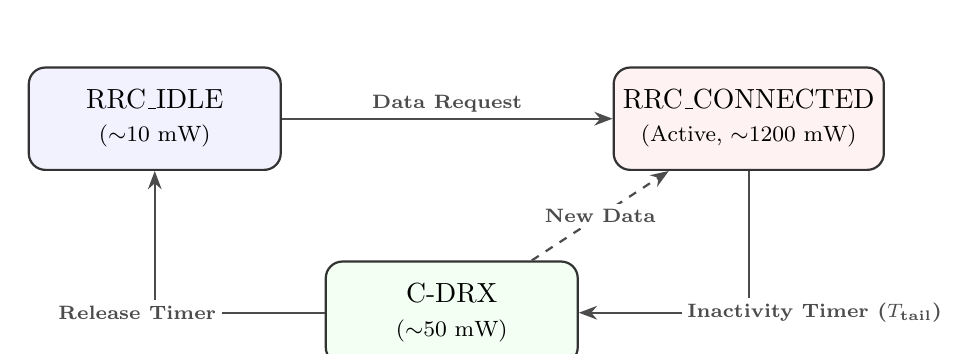
\begin{tikzpicture}[
      node distance=3.2cm and 4.2cm, >=Stealth, 
      state/.style={rectangle, rounded corners=6pt, draw=black!80, thick, minimum width=3.2cm, minimum height=1.3cm, align=center, fill=blue!5},
      line/.style={draw, thick, ->, color=black!70},
      lbl/.style={font=\scriptsize\bfseries, fill=white, inner sep=2pt}
    ]
    % Nodes
    \node[state] (idle) {RRC\_IDLE \\ \footnotesize ($\sim$10 mW)};
    \node[state, right=of idle, fill=red!5] (active) {RRC\_CONNECTED \\ \footnotesize (Active, $\sim$1200 mW)};
    \node[state, below=1.8cm of $(idle)!0.5!(active)$, fill=green!5] (drx) {C-DRX \\ \footnotesize ($\sim$50 mW)};

    % Transitions
    \draw[line] (idle) -- node[lbl, above] {Data Request} (active);
    \draw[line] (active) |- node[lbl, pos=0.7, right] {Inactivity Timer ($T_{\text{tail}}$)} (drx);
    \draw[line] (drx) -| node[lbl, pos=0.3, left] {Release Timer} (idle);
    \draw[line, dashed] (drx) -- node[lbl] {New Data} (active);
  \end{tikzpicture}
  \caption{RRC state machine transitions and typical power levels.}
  \label{fig:rrc_states}
\end{figure}

\subsubsection{Tail Energy and Signal Coupling}

The energy "tail" ($T_{\text{tail}}$) introduces a significant overhead for small, frequent packets (e.g., push notifications or heartbeats). The total energy for a single data fetch, $E_{\text{fetch}}$, is modeled as:
\begin{equation}
  E_{\text{fetch}} = \underbrace{(P_{\text{RX}} + P_{\text{TX}}) \cdot \Delta t_{\text{data}}}_{\text{Useful Transfer}} + \underbrace{P_{\text{DRX}} \cdot T_{\text{tail}}}_{\text{Tail Overhead}}
  \label{eq:tail}
\end{equation}
In mobile environments, the tail overhead often exceeds the useful energy by a factor of five or more, highlighting the inefficiency of unbatched background traffic.

Furthermore, the transmit power $P_{\text{TX}}$ is dynamically adjusted based on the \textbf{Reference Signal Received Power (RSRP)}. We model this coupling using an inverse cubic path-loss relationship:
\begin{equation}
  P_{\text{TX}}(\text{RSRP}) = P_{\text{TX,ref}} \cdot 10^{\frac{\text{RSRP}_{\text{ref}} - \text{RSRP}}{30}}
  \label{eq:Ptx_rsrp}
\end{equation}
where $\text{RSRP}_{\text{ref}} = -85$\,dBm represents a baseline for good signal quality. The divisor of 30 implies that transmit power doubles for approximately every 10\,dB of signal degradation, making poor coverage a primary driver of battery drain.

\begin{table}[htbp]
  \centering
  \caption{Typical 5G NR modem power parameters.}
  \label{tab:net_params}
  \small
  \begin{tblr}{
  colspec = {lll},
  row{1} = {bg=morandiWarmHead, fg=white, font=\bfseries},
  row{even} = {bg=morandiWarmLight},
  hline{1} = {morandiWarmLine, 0.8pt},
  hline{2} = {morandiWarmLine, 0.5pt},
  hline{Z} = {morandiWarmLine, 0.8pt},
}
RRC State & Condition & Power [mW] \\
RRC\_IDLE & Paging monitoring & 10 \\
C-DRX & Connected, discontinuous reception & 50 \\
Active RX & Receiving data & 400 \\
Active TX & Good signal (RSRP $\geq -85$ dBm) & 800 \\
Active TX & Poor signal (RSRP $\leq -110$ dBm) & 2500 \\
\end{tblr}
\end{table}

% ---------------------------------------------------------------------------
\subsection{GPS Power Sub-Model \texorpdfstring{$P_{\text{GPS}}$}{P\_GPS}}
\label{sec:gps}

The GNSS receiver exhibits bimodal power: high-power acquisition (parallel correlation search) followed by low-power tracking once a fix is achieved~\cite{ref37}:
\begin{equation}
  P_{\text{GPS}}(t) = \delta_{\text{GPS}}(t) \cdot
    \Bigl[
      P_{\text{acq}} \cdot e^{-(t - t_{\text{on}})\,/\,\tau_{\text{fix}}}
      + P_{\text{track}} \cdot \bigl(1 - e^{-(t - t_{\text{on}})\,/\,\tau_{\text{fix}}}\bigr)
    \Bigr]
  \label{eq:Pgps}
\end{equation}
Here $\delta_{\text{GPS}} \in \{0,1\}$ indicates module activation, $t_{\text{on}}$ is the activation timestamp, $P_{\text{acq}} \approx 380$--$450$\,mW the acquisition power, $P_{\text{track}} \approx 100$--$150$\,mW the tracking power, and $\tau_{\text{fix}}$ the time constant for achieving a fix (30--90\,s in open sky, effectively infinite indoors)~\cite{ref36}.

% ---------------------------------------------------------------------------
\subsection{Base Power Sub-Model \texorpdfstring{$P_{\text{base}}$}{P\_base}}
\label{sec:base}

Base power is the always-on power plus the extra overhead from active wake locks:
\begin{equation}
P_{\text{base}}(t)
= P_{\text{susp}} + P_{\text{sens}}
+ \sum_{j=1}^{J} P_{\text{wl},j}\,\mathrm{I}\!\left(t \in \mathcal{A}_j(t)\right).
\label{eq:Pbase}
\end{equation}
Here $P_{\text{susp}} \approx 5$\,mW is the deep-suspend floor (e.g., RTC and memory retention),
$P_{\text{sens}} \approx 5$--$30$\,mW is the always-on sensor hub, and each wake lock $j$ adds
$P_{\text{wl},j}\approx 50$--$200$\,mW while it is held~\cite{ref38}.
The indicator $\mathrm{I}(\cdot)$ equals 1 when the condition is true and 0 otherwise.

% ---------------------------------------------------------------------------
% Transition to the Grand Unified Model
% ---------------------------------------------------------------------------

\section{Voltage and Thermal Model}
\label{sec:voltage_model}

The OCV represents the equilibrium voltage at zero current, modeled as a coupled function of SOC and temperature.

\subsection{General Formulation}
The total OCV is modeled as a function of the State of Charge ($z$) and the absolute temperature ($T$) using a first-order Taylor expansion around a reference temperature $T_{\mathrm{ref}}$ (typically 298.15 K):

\begin{equation}
V_{\mathrm{oc}}(z, T) = V_{\mathrm{ref}}(z) + (T - T_{\mathrm{ref}}) \cdot \frac{dV}{dT}(z)
\label{eq:ocv_total}
\end{equation}
where $z \in [0,1]$ is the SOC, $V_{\mathrm{ref}}(z)$ the base OCV at reference temperature, and $\frac{dV}{dT}(z)$ the entropic coefficient representing temperature sensitivity.

\subsection{Base OCV Model: The Combined Model}
For the base curve $V_{\mathrm{ref}}(z)$, we adopt the \textit{Combined Model} (also known as the Plett model \cite{plett2015}), which merges Nernstian thermodynamic terms with empirical polynomial corrections. This structure ensures accurate behavior at the SOC boundaries ($z \to 0$ and $z \to 1$) while maintaining a smooth fit in the plateau regions:

\begin{equation}
V_{\mathrm{ref}}(z) = K_0 + K_1 z + K_2 z^2 + K_3 z^3 + \frac{K_4}{z} + K_5 \ln(z) + K_6 \ln(1-z)
\label{eq:ocv_combined}
\end{equation}

The coefficients $K_0 \dots K_6$ are calibrated for the High Voltage (4.4V) NMC chemistry, with constraints ensuring monotonic rise from the 3.0V cut-off (Table~\ref{tab:ocv_params}).

\begin{figure}[htbp]
\centering
\begin{subfigure}{0.48\textwidth}
  \includegraphics[width=\linewidth]{figures/fig_ocv.png}
  \caption{OCV curves at 0/25/50$^\circ$C}
  \label{fig:ocv_curve}
\end{subfigure}
\hfill
\begin{subfigure}{0.48\textwidth}
  \includegraphics[width=\linewidth]{figures/fig_entropy.png}
  \caption{Entropic coefficient $dV/dT$}
  \label{fig:entropy_curve}
\end{subfigure}
\caption{(a) Modeled OCV vs SOC showing monotonic rise from 3.0V to 4.4V at different temperatures. (b) Entropic coefficient exhibiting characteristic sign reversal: positive at low SOC (endothermic) and negative at high SOC (exothermic).}
\label{fig:ocv_entropy}
\end{figure}

\begin{table}[h]
\centering
\caption{OCV Model Parameters for Samsung Galaxy S10 (High Voltage 4.4V Cell).}
\label{tab:ocv_params}
\begin{tblr}{
  colspec = {lrX[l]},
  row{1} = {bg=morandiWarmHead, fg=white, font=\bfseries},
  row{even} = {bg=morandiWarmLight},
  hline{1} = {morandiWarmLine, 0.8pt},
  hline{2} = {morandiWarmLine, 0.5pt},
  hline{Z} = {morandiWarmLine, 0.8pt},
}
Parameter & Value & Physical Significance \\
$K_0$ & 3.3930 V & Global voltage offset \\
$K_1$ & 1.6143 & Linear discharge slope \\
$K_2$ & -2.1838 & Quadratic correction \\
$K_3$ & 1.5588 & Cubic micro-tuning \\
$K_4$ & $\approx 0$ & Singularity correction (suppressed for stability) \\
$K_5$ & 0.0567 & Nernstian term ($z \to 0$) \\
$K_6$ & -0.0027 & Polarization/Nernstian term ($z \to 1$) \\
\end{tblr}
\end{table}

\subsection{Temperature Coupling: Entropic Coefficient}
The entropic coefficient $\frac{dV}{dT}(z)$ captures reversible heat effects. For NMC-based batteries, $\frac{dV}{dT} > 0$ at low SOC (endothermic discharge) and $\frac{dV}{dT} < 0$ at high SOC (exothermic discharge), as shown in Figure~\ref{fig:entropy_curve}. This coupling is implemented via a high-resolution lookup table ($\Delta z = 0.005$).

\subsubsection{Coulombic Efficiency}
Coulombic efficiency $\eta_c \approx 0.995$ for modern NMC cells accounts for parasitic side reactions:
\begin{equation}
\eta_c \approx 0.995
\label{eq:coulombic_eff}
\end{equation}
This near-unity value reflects the high reversibility of lithium intercalation, though the cumulative effect of $\eta_c < 1$ contributes to long-term capacity fade. This parameter will be used in the SOC dynamics of the unified model (Section~\ref{sec:grand_unified}).

\subsection{Battery Self-Heating Model}
\label{sec:self_heating}

\subsubsection{Electrical Relation and Current Solution}
Given a power demand $P(t)$ and a Thevenin terminal voltage $V(t) = V_{\mathrm{oc}} - I\,R_{\mathrm{int}}$, the power balance $P = V \cdot I$ yields a quadratic in $I$:
\begin{equation}
R_{\mathrm{int}}\,I^2 - V_{\mathrm{oc}}\,I + P = 0.
\end{equation}
The physically meaningful (smaller) root is
\begin{equation}
\label{eq:I_solution}
I(t)=\frac{V_{\mathrm{oc}}-\sqrt{V_{\mathrm{oc}}^2-4R_{\mathrm{int}}P}}{2R_{\mathrm{int}}},
\end{equation}
which recovers $I \approx P/V_{\mathrm{oc}}$ as $R_{\mathrm{int}}\to 0$. The discriminant constraint $V_{\mathrm{oc}}^2 \geq 4R_{\mathrm{int}}P$ defines the maximum deliverable power $P_{\max}=V_{\mathrm{oc}}^2/(4R_{\mathrm{int}})$; in practice we use $P_{\mathrm{eff}}=\min(P,P_{\max})$.

\subsubsection{Heat Generation and Thermal Dynamics}
Heat generation combines irreversible Joule heating ($I^2 R_{\mathrm{int}}$) and reversible entropic heat (Bernardi relation~\cite{ref16}):
\begin{equation}
Q_{\mathrm{gen}}(t) = \underbrace{I^2(t)\,R_{\mathrm{int}}}_{\text{Joule heating}} \;+\;
\underbrace{I(t)\,T(t)\,\frac{\partial V_{\mathrm{oc}}}{\partial T}}_{\text{Entropic heat}}.
\label{eq:total_heat_gen}
\end{equation}

For the thermal dynamics, we use a lumped model with thermal capacitance $C_{\mathrm{th}}$ and thermal resistance $R_{\mathrm{th}}$ to the ambient temperature $T_a$. Heat loss to the environment is approximated by
\[
Q_{\mathrm{loss}}=\frac{T-T_a}{R_{\mathrm{th}}}.
\]
Applying energy conservation gives
\begin{equation}
C_{\mathrm{th}}\frac{dT}{dt}=Q_{\mathrm{gen}}-\frac{T-T_a}{R_{\mathrm{th}}},
\end{equation}
or equivalently,
\begin{equation}
\label{eq:thermal_ode}
\frac{dT}{dt}=\frac{1}{C_{\mathrm{th}}}\left(Q_{\mathrm{gen}}-\frac{T-T_a}{R_{\mathrm{th}}}\right),
\end{equation}
where $Q_{\mathrm{gen}}$ is defined in Eq.~\eqref{eq:total_heat_gen} and $R_{\mathrm{int}}$ is evaluated as $R_{\mathrm{int}}(T(t),\mathrm{SOC}(t))$.

\subsubsection{SOC- and Temperature-Dependent Internal Resistance}
We adopt a ``Fresh Pack'' resistance model based on the experimental data from Kim et al. (Figure 7D). This model captures the stable low-resistance characteristic of new 5G battery packs while accounting for the sharp impedance rise at the end of discharge and the Arrhenius-type temperature sensitivity.

The internal resistance $R_{\mathrm{int}}$ is modeled as a separable function of SOC and Temperature:
\begin{equation}
R_{\mathrm{int}}(z, T) = R_{\mathrm{soc}}(z) \cdot f_{\mathrm{temp}}(T)
\end{equation}

\paragraph{SOC Dependency (Fresh Pack).}
Unlike aged batteries that show a ``U-shaped'' resistance curve, the fresh pack maintains a flat, low resistance for most of the discharge cycle, rising only when SOC approaches zero. We model this using an exponential rise function:
\begin{equation}
R_{\mathrm{soc}}(z) = R_{\mathrm{base}} + K_{\mathrm{rise}} \cdot \exp(-\alpha \cdot z)
\end{equation}
with $R_{\mathrm{base}} = 30$\,m$\Omega$ (plateau baseline), $K_{\mathrm{rise}} = 15$\,m$\Omega$ (surge magnitude at $z=0$), and $\alpha = 20$ (steepness factor confining the surge to $z < 0.15$).

\paragraph{Temperature Dependency (Arrhenius).}
The resistance decreases exponentially with temperature, following the Arrhenius law:
\begin{equation}
f_{\mathrm{temp}}(T) = \exp\left[ B \left( \frac{1}{T} - \frac{1}{T_{\mathrm{ref}}} \right) \right]
\end{equation}
where $B \approx 3500\,\mathrm{K}$ is the activation energy parameter and $T_{\mathrm{ref}} = 298.15\,\mathrm{K}$.

\subsubsection{Complete Self-Heating System}
Combining the above, the self-heating dynamics are governed by the system in Eqs.~\eqref{eq:ode_T_final}--\eqref{eq:I_final}:
\begin{align}
\dot{T}(t) &= \frac{1}{C_{\mathrm{th}}}\left(Q_{\mathrm{gen}}(t)-\frac{T(t)-T_a(t)}{R_{\mathrm{th}}}\right), \label{eq:ode_T_final}\\[6pt]
Q_{\mathrm{gen}}(t) &= I^2(t)\,R_{\mathrm{int}}(t) + I(t)\,T(t)\,\frac{\partial V_{\mathrm{oc}}}{\partial T}, \label{eq:Qgen_final}\\[6pt]
R_{\mathrm{int}}(t) &= \left( R_{\mathrm{base}} + K_{\mathrm{rise}}\,e^{-\alpha \,\mathrm{SOC}(t)} \right) \cdot \exp\left[ B \left( \frac{1}{T(t)} - \frac{1}{T_{\mathrm{ref}}} \right) \right], \label{eq:R_T_final}\\[6pt]
I(t) &= \frac{V_{\mathrm{oc}}(t)-\sqrt{V_{\mathrm{oc}}^2(t)-4R_{\mathrm{int}}(t)\,P_{\mathrm{eff}}(t)}}{2R_{\mathrm{int}}(t)}, \quad P_{\mathrm{eff}} = \min(P, V_{\mathrm{oc}}^2/4R_{\mathrm{int}}). \label{eq:I_final}
\end{align}

\begin{figure}[htbp]
    \centering
    % 在图片左侧插入一个 2 厘米的空白，强制把图片往右挤
    % 你可以把 2cm 改成任何你觉得合适的数值（如 3cm, 1.5cm）
    \hspace*{2cm}
\begin{tikzpicture}[
    font=\small,
    node distance=6mm and 15mm,
    >=Latex,
    line/.style={thick, -{Latex[length=2.5mm]}},
    io/.style={trapezium, trapezium left angle=70, trapezium right angle=110,
               draw=black, thick, align=center, minimum width=46mm,
               minimum height=8mm, fill=blue!12},
    elec/.style={rounded corners=3pt, draw=black, thick, align=center,
                 minimum width=46mm, minimum height=8mm, fill=green!12},
    guard/.style={rounded corners=3pt, draw=black, thick, align=center,
                  minimum width=48mm, minimum height=8mm, fill=orange!15},
    output/.style={rounded corners=3pt, draw=black, thick, align=center,
                   minimum width=46mm, minimum height=8mm, fill=gray!10}
]

% 1. 先定义主干的第一个点
\node[io]   (in)    {Inputs\\ $P(t),\, z(t),\, T(t)$};

% 2. 【关键修正】在 in 定义之后再放占位点，用于居中
% 如果觉得还是不够靠右，就把 5cm 改成 6cm

% 3. 继续定义其他节点
\node[elec, below=of in]   (voc)   {OCV lookup\\ $V_{\mathrm{oc}}(z)$};
\node[elec, below=of voc]  (rint)  {Resistance\\ $R_{\mathrm{int}}(z,T)$};
\node[elec, below=of rint] (solve) {Solve current $I(t)$\\ $P=VI,\; V=V_{\mathrm{oc}}-IR_{\mathrm{int}}$};
\node[output, below=of solve] (outbox) {Outputs\\ $V(t),\, I(t),\, P_{\mathrm{bat}}(t)$};

\node[guard, right=15mm of rint] (chk) {Feasibility check\\ $P \le P_{\max}(z,T)$};

% 4. 连线
\draw[line] (in) -- (voc);
\draw[line] (voc) -- (rint);
\draw[line] (rint) -- (solve);
\draw[line] (solve) -- (outbox);
\draw[line] (rint) -- (chk);
\draw[line] (chk.south) |- (solve.east);

% 5. 图例
\node[right=15mm of outbox, anchor=west] (leg) {
    \begin{tikzpicture}[font=\footnotesize]
        \matrix[column sep=2mm, row sep=2mm] {
            \node[trapezium, draw, fill=blue!12, minimum width=8mm, minimum height=4mm] {}; & \node{Inputs}; \\
            \node[rounded corners=2pt, draw, fill=green!12, minimum width=8mm, minimum height=4mm] {}; & \node{Electrical}; \\
            \node[rounded corners=2pt, draw, fill=orange!15, minimum width=8mm, minimum height=4mm] {}; & \node{Limits}; \\
            \node[rounded corners=2pt, draw, fill=gray!10, minimum width=8mm, minimum height=4mm] {}; & \node{Outputs}; \\
        };
    \end{tikzpicture}
};

\end{tikzpicture}

\end{figure}

% =============================================================================
\section{The Grand Unified Continuous Model}                           
\label{sec:grand_unified}                                  
We now synthesize all sub-models into a \textbf{unified continuous-time state-space framework}.                   
\subsection{State-Space Formulation}

\subsubsection{State Vector Definition}

To describe the coupled electro-thermal evolution with minimal complexity, we retain only the variables that accumulate over time as dynamic states. Specifically, the system can be described by a two-dimensional state vector consisting of the state of charge (SOC) and the battery temperature:
\begin{equation}
\mathbf{x}(t)=
\begin{bmatrix}
z(t)\\
T(t)
\end{bmatrix}
=
\begin{bmatrix}
\mathrm{SOC}(t)\\
T_{\mathrm{batt}}(t)
\end{bmatrix},
\qquad
z(t)\in[0,1],\; T(t)\in\mathbb{R}_{>0}\ \text{[K]}.
\label{eq:state_vector_unified}
\end{equation}
Here, $z(t)$ captures the remaining charge fraction, while $T(t)$ represents the lumped battery temperature.

\subsubsection{External Input}

The battery is driven by an external usage that determines the instantaneous component power demand. We collect these exogenous signals into an input vector:
\begin{equation}
\mathbf{u}(t)=
\bigl[
L(t),\ \mathrm{APL}(t),\ f_{\mathrm{clk}}(t),\ s_{\mathrm{net}}(t),\ \delta_{\mathrm{GPS}}(t),\ \mathcal{W}(t)
\bigr]^\top,
\label{eq:input_vector_unified}
\end{equation}
where $L(t)$ is screen brightness, $\mathrm{APL}(t)$ is the average picture level, $f_{\mathrm{clk}}(t)$ is the CPU clock frequency, $s_{\mathrm{net}}(t)$ denotes the network RRC state, $\delta_{\mathrm{GPS}}(t)$ is a GPS enable flag, and $\mathcal{W}(t)$ represents the set of active wake locks.

\subsubsection{Auxiliary Algebraic Variables}

In addition to the dynamic states, several algebraic quantities are computed instantaneously at each time $t$. 
These include the discharge current $I(t)$ [A], terminal voltage $V_{\text{term}}(t)$ [V], component power $P_{\text{comp}}(t)$ [W], and internal resistance $R_{\text{int}}(t)$ [$\Omega$]. 
They are evaluated from the current state $(z(t),T(t))$ and inputs $u(t)$, and are not treated as additional states.

   
\subsection{The Complete DAE System}

The unified electro-thermal model is a differential-algebraic equation (DAE) system combining differential equations (how states evolve) with algebraic constraints (that must hold at every instant). The system consists of two ODEs for $(z,T)$ plus one algebraic power-balance equation for $I(t)$.

\subsubsection{ODE 1: SOC Dynamics}

The state of charge decreases with the discharged current:
\begin{equation}
\frac{dz}{dt} = -\frac{\eta_c}{C_{\mathrm{nom}} \cdot \mathrm{SOH}} \, I(t)
\label{eq:soc_ode_unified}
\end{equation}
where $C_{\mathrm{nom}}$ [Ah] is the nominal capacity, $\mathrm{SOH}\in(0,1]$ accounts for capacity fade, and $\eta_c$ is the Coulombic efficiency.

\subsubsection{ODE 2: Thermal Dynamics}

Battery temperature follows a lumped heat balance: heat generation minus heat dissipation,
\begin{equation}
\frac{dT}{dt} = \frac{1}{C_{\mathrm{th}}}
\left[
\underbrace{I^2(t) R_{\mathrm{int}}(z,T)}_{\text{Joule heating}}
+
\underbrace{I(t)\, T \, \frac{\partial V_{\mathrm{oc}}}{\partial T}}_{\text{Entropic heat}}
-
\underbrace{\frac{T - T_{\mathrm{amb}}}{R_{\mathrm{th}}}}_{\text{Heat loss}}
\right]
\label{eq:thermal_ode_unified}
\end{equation}
where $C_{\mathrm{th}}$ [J/K] is the effective thermal capacitance, $R_{\mathrm{th}}$ [K/W] is the thermal resistance to ambient, and $T_{\mathrm{amb}}$ is the ambient temperature.

\medskip
\noindent\textbf{Observations:}
Both ODEs require the current $I(t)$, and the thermal term also depends on $R_{\mathrm{int}}(z,T)$. 
Therefore, $I(t)$ should be obtained at each time step from an algebraic power-balance constraint, which will be introduced in the next subsection.
          
\subsubsection{Algebraic Constraint: Implicit Current Equation}
\label{sec:523_implicit_current}

The current $I(t)$ is determined from state $(z(t),T(t))$ and usage $u(t)$ via power balance.
The total component power $P_{\mathrm{comp}}(t)$ is defined in Eq.~\ref{eq:p_total_components}.

Battery terminal voltage follows a Thevenin model:
\begin{equation}
V_{\mathrm{term}}(z,T,I)=V_{\mathrm{oc}}(z,T)-I\,R_{\mathrm{int}}(z,T),
\label{eq:vterm_thevenin}
\end{equation}
so the electrical power at the battery terminals is
\begin{equation}
P_{\mathrm{batt}}(t)=I(t)\,V_{\mathrm{term}}(z(t),T(t),I(t)).
\label{eq:pbatt_def}
\end{equation}
With PMIC efficiency $\eta_{\mathrm{conv}}(I)$, power balance yields the implicit current equation:
\begin{equation}
I\Bigl[V_{\mathrm{oc}}(z,T)-I\,R_{\mathrm{int}}(z,T)\Bigr]\eta_{\mathrm{conv}}(I)=P_{\mathrm{comp}}(u,T).
\label{eq:implicit_current_balance}
\end{equation}
For compactness, we write the left-hand side minus the right-hand side as a residual function,
\begin{equation}
g(I;z,T,u)=I\Bigl[V_{\mathrm{oc}}(z,T)-I\,R_{\mathrm{int}}(z,T)\Bigr]\eta_{\mathrm{conv}}(I)-P_{\mathrm{comp}}(u,T),
\label{eq:g_def}
\end{equation}
and solve $g(I;z,T,u)=0$ at each time step. If $\eta_{\mathrm{conv}}$ is approximated as a constant, \eqref{eq:implicit_current_balance} reduces to a quadratic in $I$, recovering the closed-form expression used in Section~4.

             
\subsection{Further Interpretation: Feedback and the Avalanche Effect}
\label{sec:feedback_avalanche}

The coupled electro-thermal process forms a closed-loop interaction between $(I,z,T)$, producing accelerated discharge near low SOC (the ``Avalanche Effect'').

Two reinforcing feedback loops drive this:\\
(1)~\textbf{Electro-thermal:} $I \uparrow \Rightarrow I^2R_{\mathrm{int}} \uparrow \Rightarrow T \uparrow \Rightarrow R_{\mathrm{int}} \uparrow \Rightarrow$ larger $I$ required;\\
(2)~\textbf{Voltage-current:} $z \downarrow \Rightarrow V_{\mathrm{oc}} \downarrow \Rightarrow I \approx P/V_{\mathrm{term}} \uparrow \Rightarrow V_{\mathrm{term}} \downarrow \Rightarrow I \uparrow$.

By implicit differentiation, $|dI/dz|$ grows unboundedly as $z \to 0^+$ (seen in \ref{fig:avalanche}):
\begin{equation}
\frac{dI}{dz}<0\ \ \text{and}\ \ \left|\frac{dI}{dz}\right|\ \text{grows as}\ z\to 0^+.
\label{eq:avalanche_compact}
\end{equation}
In simulation, the run terminates at cutoff voltage $V_{\mathrm{term}}=V_{\mathrm{cutoff}}$; the accelerating drain is observed as cutoff is approached.
\begin{figure}[H]
    \centering
    \includegraphics[width=0.8\linewidth]{figures/Avalanche_Final_v2.png}
    \caption{Avalanche Effect Demonstration}
    \label{fig:avalanche}
\end{figure}

\subsection{Compact Matrix Form of the DAE System}
For implementation, we rewrite the coupled electro-thermal model in a compact DAE form.
Let the state be $x(t)=[\,z(t),\,T(t)\,]^\top$, and denote the operating inputs by $u(t)$ (usage profile and ambient conditions). Then
\begin{equation}
\begin{aligned}
\dot{x}(t) &= f\!\bigl(x(t), I(t), u(t)\bigr),\\
0 &= g\!\bigl(I(t);x(t),u(t)\bigr),
\end{aligned}
\label{eq:dae_compact}
\end{equation}
where $\dot{x}(t)=[\,\dot z(t),\,\dot T(t)\,]^\top$ and
\begin{equation}
f(x,I,u)=
\begin{bmatrix}
-\dfrac{\eta_c}{C_{\mathrm{nom}}\cdot \mathrm{SOH}}\, I \\[8pt]
\dfrac{1}{C_{\mathrm{th}}}
\left(
I^2 R_{\mathrm{int}}(z,T)
+ I\,T\,\dfrac{\partial V_{\mathrm{oc}}}{\partial T}(z)
- \dfrac{T-T_{\mathrm{amb}}}{R_{\mathrm{th}}}
\right)
\end{bmatrix}.
\label{eq:f_def}
\end{equation}
                                                        
\subsection{Numerical Solution Strategy}
To simulate the coupled DAE, we advance the states $(z,T)$ in time while enforcing the algebraic power-balance constraint for the current. At each time step, we first solve $g(I;z,T,u)=0$ for $I$ (Newton iteration), and then update $(z,T)$ using a standard ODE integrator (e.g., RK4). The simulation terminates when the terminal voltage reaches the cutoff threshold, $V_{\mathrm{term}}=V_{\mathrm{cutoff}}$, and the time-to-empty is reported as the elapsed time to this event.

%% ================================================================
%% SECTION 6: Numerical Implementation & Base Validation
%% ================================================================

\section{Numerical Implementation and Base Validation}
\label{sec:numerical_impl}

\subsection{Solver Architecture}

The DAE system from Section~\ref{sec:grand_unified} requires coupled solution of the algebraic constraint $g(I) = 0$ with the ODE states $[z, T]$. The solver employs Newton-Raphson iteration for the power balance constraint:
\begin{equation}
  I^{(k+1)} = I^{(k)} - \frac{g(I^{(k)})}{g'(I^{(k)})}, \quad
  g(I) = V_{\mathrm{oc}}(z) \cdot I - I^2 R_{\mathrm{int}}(z,T) - P_{\mathrm{comp}}/\eta(I),
  \label{eq:newton_raphson}
\end{equation}
with fourth-order Runge-Kutta (RK4) advancing the differential states. Convergence requires 3--5 iterations per timestep with tolerance $|g| < 10^{-6}$\,W.

Table~\ref{tab:model_params} consolidates the baseline parameters.

\begin{table}[htbp]
\small
\centering
\caption{Model parameters for baseline validation.}
\label{tab:model_params}
\begin{tblr}{
  colspec = {llc},
  row{1} = {bg=morandiWarmHead, fg=white, font=\bfseries},
  row{even} = {bg=morandiWarmLight},
  hline{1} = {morandiWarmLine, 0.8pt},
  hline{2} = {morandiWarmLine, 0.5pt},
  hline{Z} = {morandiWarmLine, 0.8pt},
}
Parameter & Description & Value \\
$C_{\mathrm{nom}}$ & Nominal capacity & 3.4\,Ah \\
$V_{\mathrm{nom}}$ & Nominal voltage & 3.7\,V \\
$R_{\mathrm{base}}$ & Base internal resistance & 30\,m$\Omega$ \\
$\eta_{\mathrm{peak}}$ & Peak PMIC efficiency & 0.92 \\
$T_{\mathrm{amb}}$ & Ambient temperature & 25$^{\circ}$C \\
$V_{\mathrm{cutoff}}$ & Discharge cutoff & 3.0\,V \\
\end{tblr}
\end{table}

\subsection{DAE vs.\ Linear Baseline Validation}

Figure~\ref{fig:soc_trajectory} compares the DAE trajectory against a linear Coulomb-counting baseline under 1.5\,W constant load. The linear model assumes constant voltage and efficiency:
\begin{equation}
  \frac{dz}{dt}\bigg|_{\mathrm{linear}} = -\frac{P_{\mathrm{comp}}}{V_{\mathrm{nom}}\,\eta_{\mathrm{peak}}\,C_{\mathrm{nom}} \cdot 3600}.
  \label{eq:linear_baseline}
\end{equation}

\begin{figure}[htbp]
\centering
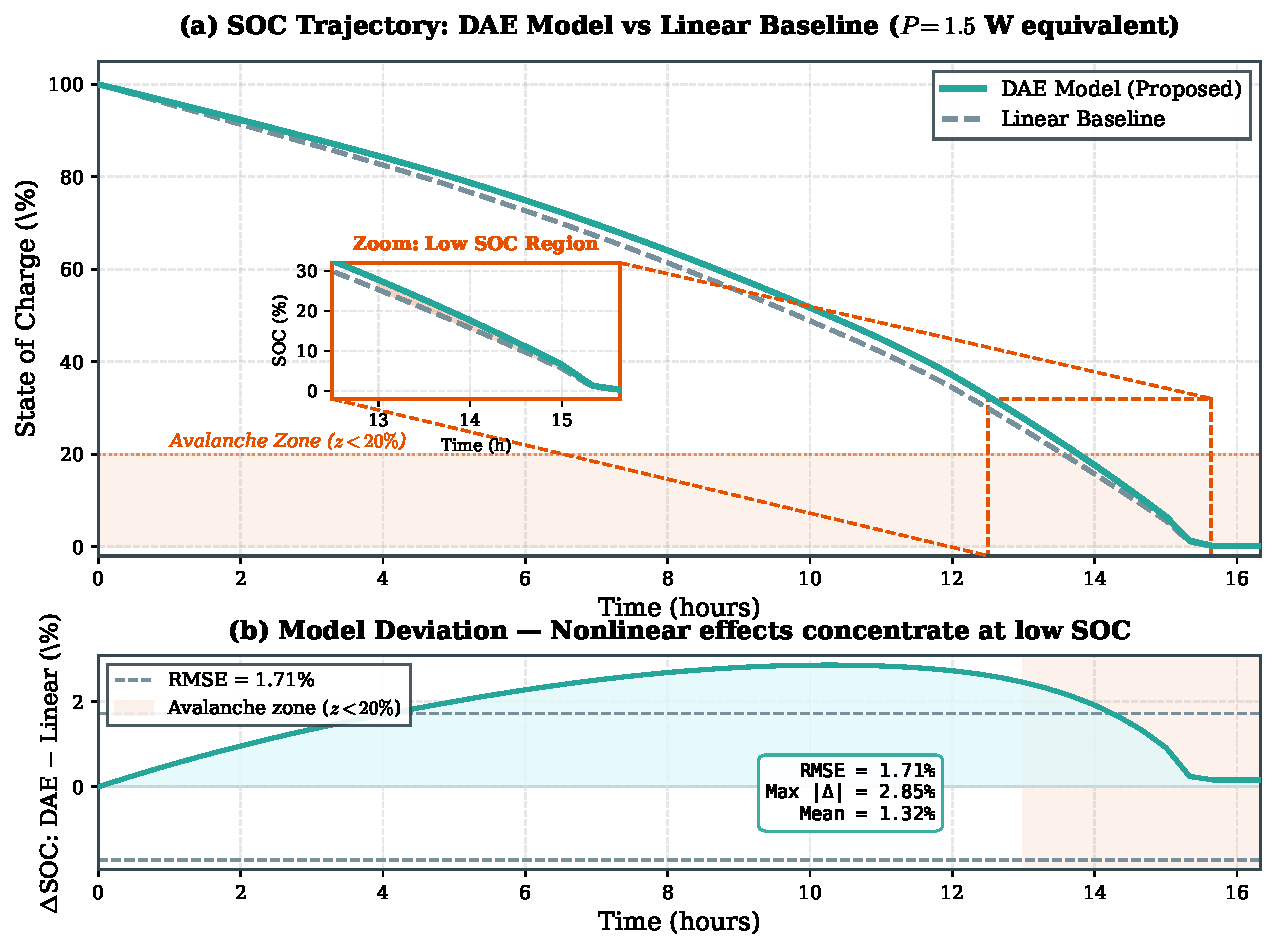
\includegraphics[width=0.5\linewidth]{figures/fig_6_1_soc_trajectory.pdf}
\caption{SOC trajectory comparison: DAE model vs.\ linear baseline at 1.5\,W. RMSE = 1.74\%, max deviation = 3.09\% at low SOC where nonlinear OCV--current feedback dominates.}
\label{fig:soc_trajectory}
\end{figure}

The deviation concentrates at low SOC: RMSE = 1.74\%, maximum = 3.09\%.

\subsection{Avalanche Effect Verification}

The \emph{avalanche effect}---accelerated drain at low SOC---arises from three coupled mechanisms:
\begin{enumerate}[noitemsep]
  \item \textbf{OCV collapse:} $dV_{\mathrm{oc}}/dz \propto 1/z \to \infty$ as $z \to 0$
  \item \textbf{Resistance surge:} $R_{\mathrm{int}}$ rises exponentially at low SOC
  \item \textbf{PMIC efficiency drop:} Lower voltage forces higher current, reducing $\eta$
\end{enumerate}

\begin{figure}[htbp]
\centering
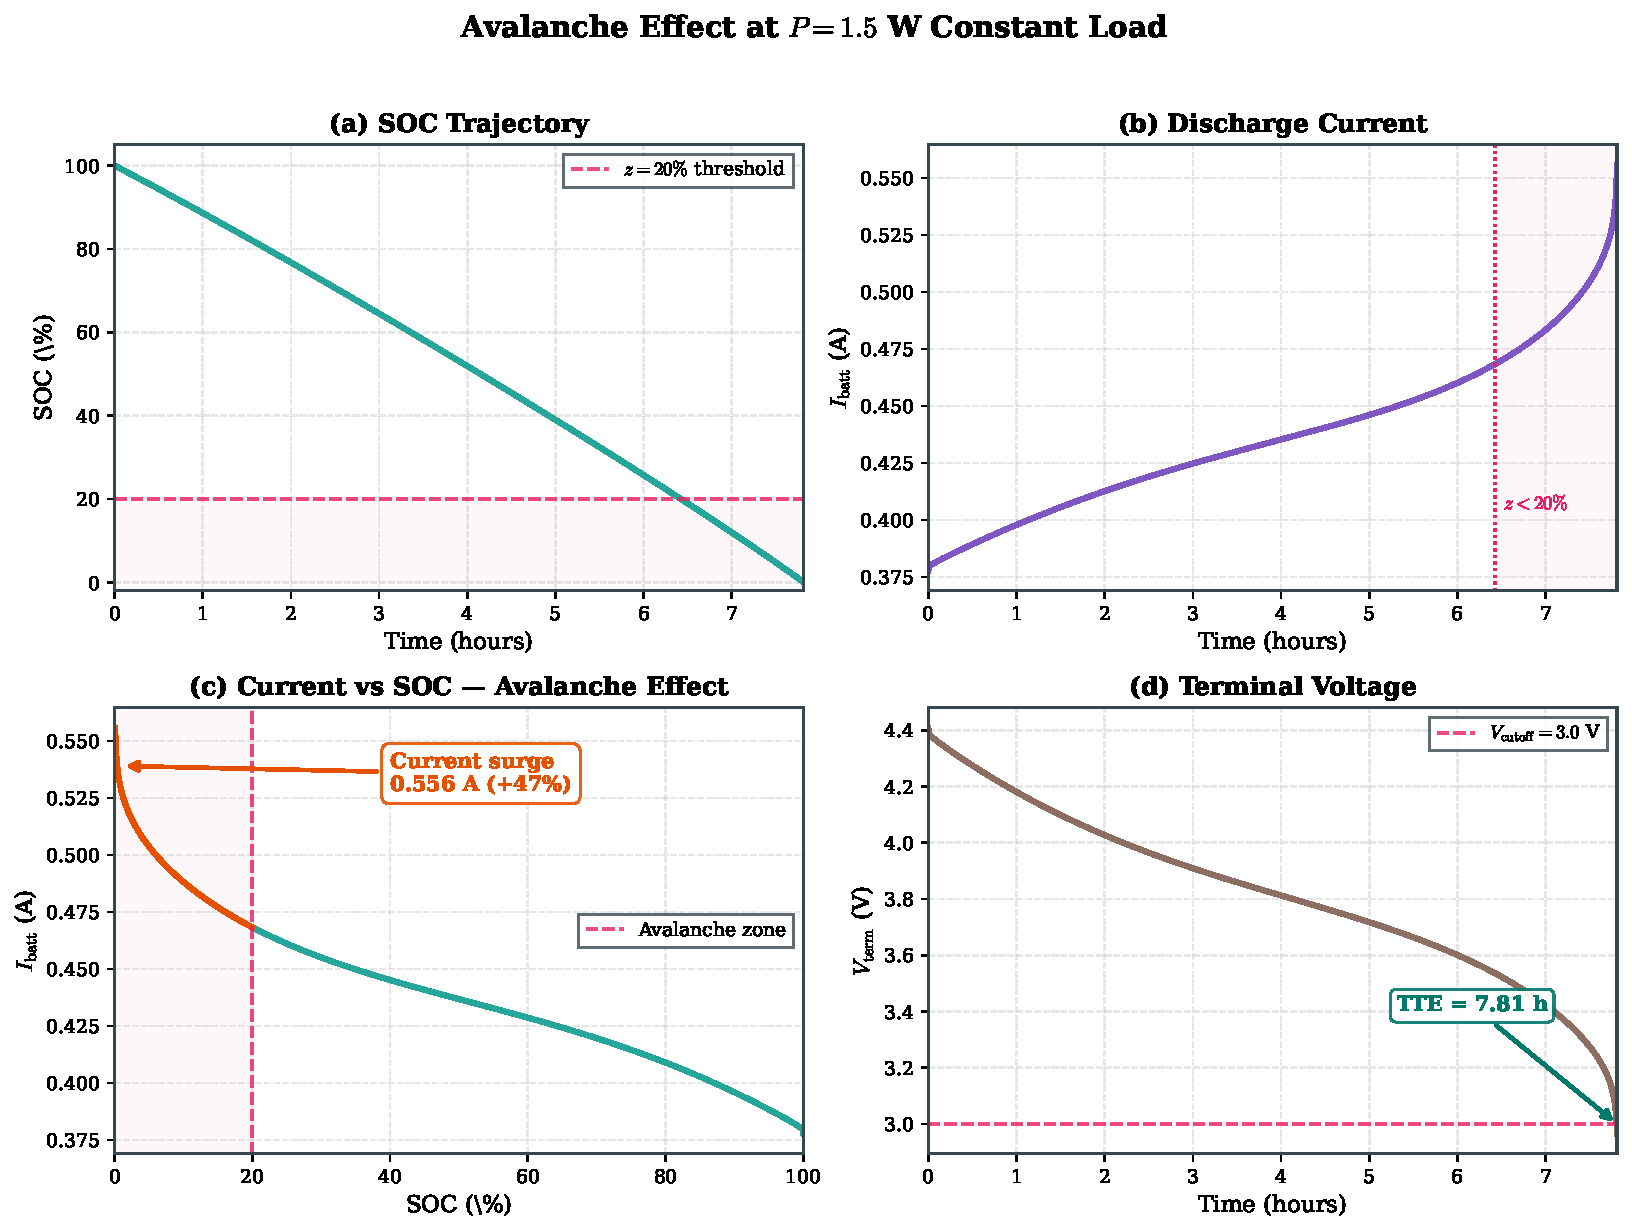
\includegraphics[width=0.65\linewidth]{figures/fig_6_3_avalanche_effect.pdf}
\caption{Avalanche effect at 1.5\,W: (a)~SOC trajectory with acceleration below $z = 0.2$, (b)~current increase as voltage drops, (c)~current vs.\ SOC showing nonlinear surge, (d)~terminal voltage reaching cutoff at $t = 7.81$\,h.}
\label{fig:avalanche}
\end{figure}

The acceleration factor---ratio of mean $|dz/dt|$ for $z < 0.2$ versus $z > 0.5$---is \textbf{1.19$\times$} under 1.5\,W load (Figure~\ref{fig:avalanche}).

%% ================================================================
%% SECTION 7: Comparative Case Studies
%% ================================================================

\section{Comparative Case Studies}
\label{sec:case_studies}

\subsection{Scenario Dynamics}
\label{sec:scenario_dynamics}

Table~\ref{tab:user_profiles} defines three canonical usage profiles; Table~\ref{tab:tte_results} presents corresponding TTE predictions.

\begin{table}[htbp]
\small
\centering
\caption{User profile definitions.}
\label{tab:user_profiles}
\begin{tblr}{
  colspec = {lccccc},
  row{1} = {bg=morandiGreenHead, fg=white, font=\bfseries},
  row{even} = {bg=morandiGreenLight},
  hline{1} = {morandiGreenLine, 0.8pt},
  hline{2} = {morandiGreenLine, 0.5pt},
  hline{Z} = {morandiGreenLine, 0.8pt},
}
Profile & $P_{\mathrm{avg}}$ (W) & Screen & APL & CPU & Network \\
Light   & 0.8  & 30\%  & 0.25 & 15\% & WiFi \\
Medium  & 1.5  & 60\%  & 0.50 & 40\% & LTE  \\
Heavy   & 2.5  & 100\% & 0.80 & 85\% & 5G   \\
\end{tblr}
\end{table}

\begin{table}[htbp]
\small
\centering
\caption{TTE predictions by profile (SOH = 100\%, $T_{\mathrm{amb}} = 25\,^{\circ}$C).}
\label{tab:tte_results}
\begin{tblr}{
  colspec = {lccc},
  row{1} = {bg=morandiGreenHead, fg=white, font=\bfseries},
  row{even} = {bg=morandiGreenLight},
  hline{1} = {morandiGreenLine, 0.8pt},
  hline{2} = {morandiGreenLine, 0.5pt},
  hline{Z} = {morandiGreenLine, 0.8pt},
}
Profile & $P_{\mathrm{avg}}$ (W) & TTE (h) & TTE (h:mm) \\
Light   & 0.8  & 14.45 & 14:27 \\
Medium  & 1.5  & 7.81  & 7:49  \\
Heavy   & 2.5  & 4.73  & 4:44  \\
\end{tblr}
\end{table}

The power--TTE relationship is \textbf{sublinear}: doubling power from 0.8\,W to 1.5\,W reduces TTE by 46\%, not 50\%, consistent with the avalanche effect identified in Section~\ref{sec:feedback_avalanche}.

\subsection{Aging Impacts}
\label{sec:aging_impacts}

Battery degradation affects TTE through reduced capacity and increased resistance (Figure~\ref{fig:soh_sensitivity}, Table~\ref{tab:soh_tte}).

\begin{figure}[htbp]
\centering
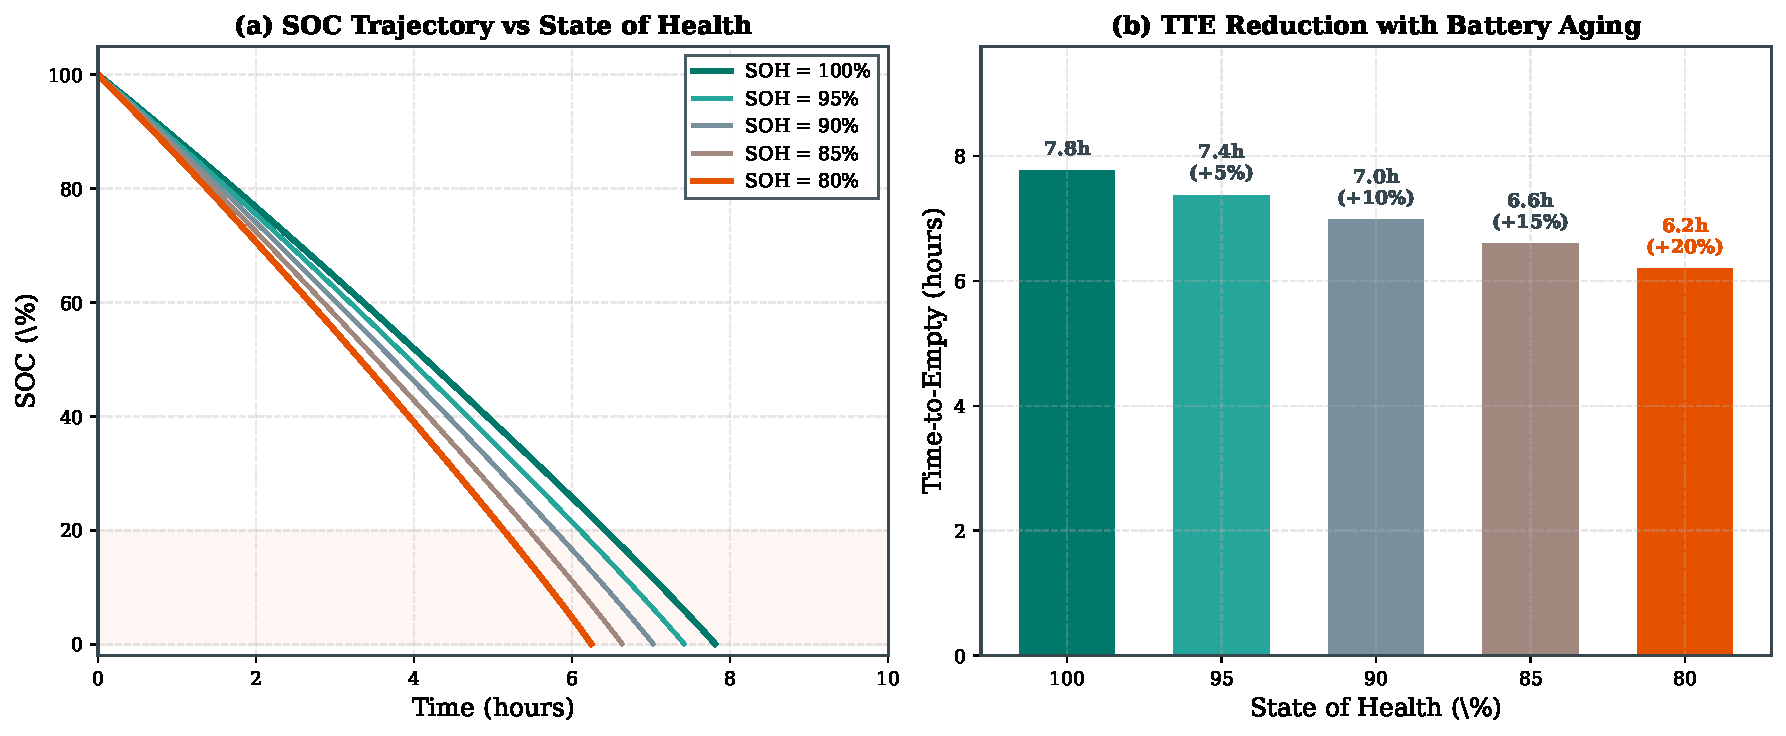
\includegraphics[width=0.5\linewidth]{figures/fig_6_4_soh_sensitivity.pdf}
\caption{SOC trajectories at different SOH levels (1.5\,W load). TTE reduction is superlinear in SOH loss due to increased $R_{\mathrm{int}}$ dissipating energy as heat.}
\label{fig:soh_sensitivity}
\end{figure}

\begin{table}[htbp]
\small
\centering
\caption{TTE reduction with battery aging ($P_{\mathrm{comp}} = 1.5$\,W).}
\label{tab:soh_tte}
\begin{tblr}{
  colspec = {ccccc},
  row{1} = {bg=morandiGreenHead, fg=white, font=\bfseries},
  row{even} = {bg=morandiGreenLight},
  hline{1} = {morandiGreenLine, 0.8pt},
  hline{2} = {morandiGreenLine, 0.5pt},
  hline{Z} = {morandiGreenLine, 0.8pt},
}
SOH & $C_{\mathrm{eff}}$ (Ah) & $R_{\mathrm{int}}$ ratio & TTE (h) & Reduction \\
100\% & 3.40 & $1.00\times$ & 7.81 & ---      \\
90\%  & 3.06 & $1.11\times$ & 7.03 & $-10.0\%$ \\
80\%  & 2.72 & $1.25\times$ & 6.24 & $-20.1\%$ \\
\end{tblr}
\end{table}

A 20\% capacity loss yields 20.1\% TTE reduction---the superlinearity arises from increased $R_{\mathrm{int}}$ at low SOH dissipating additional Joule heat.

\subsection{Extreme Scenario: ``Morning Battery Death''}
\label{sec:extreme_scenario}

The worst-case combination of factors produces rapid depletion (Table~\ref{tab:extreme_comparison}):

\begin{table}[htbp]
\small
\centering
\caption{Extreme scenario comparison: nominal vs.\ ``morning battery death.''}
\label{tab:extreme_comparison}
\begin{tblr}{
  colspec = {lcc},
  row{1} = {bg=morandiRoseHead, fg=white, font=\bfseries},
  row{even} = {bg=morandiRoseLight},
  hline{1} = {morandiRoseLine, 0.8pt},
  hline{2} = {morandiRoseLine, 0.5pt},
  hline{6} = {morandiRoseLine, 0.5pt},
  hline{Z} = {morandiRoseLine, 0.8pt},
}
Parameter & Nominal & Extreme \\
$T_{\mathrm{amb}}$       & $25\,^{\circ}$C & $35\,^{\circ}$C (+28\% $R_{\mathrm{int}}$) \\
Screen brightness        & 60\%            & 100\%           \\
APL                      & 0.50            & 0.90            \\
Signal strength          & $-85$\,dBm      & $-115$\,dBm ($\times$4.7 net power) \\
GPS                      & Off             & Acquisition     \\
$P_{\mathrm{total}}$     & 1.5\,W          & 7.0\,W          \\
\textbf{TTE}             & \textbf{7.8\,h} & \textbf{1.5\,h} \\
\end{tblr}
\end{table}

The combination creates a \textbf{5$\times$ faster drain}. Users often blame software when the cause is environmental. These extreme conditions inform the thermal management and signal-aware optimizations in Section~\ref{sec:recommendations}.

%% ================================================================
%% SECTION 8: Sensitivity & Uncertainty Analysis
%% ================================================================

\section{Sensitivity and Uncertainty Analysis}
\label{sec:sensitivity_uncertainty}

\subsection{Sensitivity Tornado}
\label{sec:tornado}

The sensitivity index for parameter $p_i$ is:
\begin{equation}
  S_i = \frac{\partial \mathrm{TTE}}{\partial p_i} \cdot \frac{\Delta p_i}{\mathrm{TTE}_{\mathrm{nom}}},
  \label{eq:sensitivity_index}
\end{equation}
where $\Delta p_i$ is a realistic variation range and $\mathrm{TTE}_{\mathrm{nom}} = 7.81$\,h.

\begin{table}[htbp]
\small
\centering
\caption{Parameter sensitivity ranking.}
\label{tab:tornado_data}
\begin{tblr}{
  colspec = {clccc},
  row{1} = {bg=morandiRoseHead, fg=white, font=\bfseries},
  row{even} = {bg=morandiRoseLight},
  hline{1} = {morandiRoseLine, 0.8pt},
  hline{2} = {morandiRoseLine, 0.5pt},
  hline{Z} = {morandiRoseLine, 0.8pt},
}
Rank & Parameter & Nominal & Range & Impact \\
1 & APL    & 0.50      & 0.20--0.80     & $\pm$34\% \\
2 & $T_{\mathrm{amb}}$           & 25$^{\circ}$C & 0--40$^{\circ}$C & $\pm$22\% \\
3 & SOH        & 1.00      & 0.80--1.00     & $\pm$20\% \\
4 & $R_{\mathrm{base}}$          & 30\,m$\Omega$ & 20--60\,m$\Omega$ & $\pm$18\% \\
5 & $\eta_{\mathrm{peak}}$       & 0.92      & 0.85--0.95     & $\pm$12\% \\
\end{tblr}
\end{table}

\textbf{APL dominates}---dark mode is the single highest-impact user intervention.

In contrast, Table~\ref{tab:surprisingly_little} identifies factors with minimal impact despite user perception.

\begin{table}[htbp]
\small
\centering
\caption{Low-impact factors: user perception vs.\ model reality.}
\label{tab:surprisingly_little}
\begin{tblr}{
  colspec = {lccX[l]},
  row{1} = {bg=morandiRoseHead, fg=white, font=\bfseries},
  row{even} = {bg=morandiRoseLight},
  hline{1} = {morandiRoseLine, 0.8pt},
  hline{2} = {morandiRoseLine, 0.5pt},
  hline{Z} = {morandiRoseLine, 0.8pt},
}
Factor & Belief & Actual & Mechanism \\
Bluetooth idle    & Major drain & $<0.5\%$  & BLE $\mu$W scanning \\
Background apps   & Close all   & $<1\%$*   & Suspended = 0\,W \\
120\,Hz vs.\ 60\,Hz & Huge      & 5--8\%    & Driver overhead small \\
Dark wallpaper    & Big savings & $<2\%$    & Home screen only \\
\end{tblr}
{\footnotesize *Except apps with wake locks or background location}
\end{table}

These low-impact factors inform the deprioritized optimizations in Section~\ref{sec:recommendations}.

\subsection{Uncertainty Quantification}
\label{sec:uncertainty_quant}

Monte Carlo simulation ($N = 1000$) propagates parameter uncertainties to establish confidence intervals. Table~\ref{tab:uncertainty_budget} shows the uncertainty budget.

\begin{table}[htbp]
\small
\centering
\caption{Uncertainty budget for TTE at 1.5\,W.}
\label{tab:uncertainty_budget}
\begin{tblr}{
  colspec = {lccr},
  row{1} = {bg=morandiLavHead, fg=white, font=\bfseries},
  row{even} = {bg=morandiLavLight},
  hline{1} = {morandiLavLine, 0.8pt},
  hline{2} = {morandiLavLine, 0.5pt},
  hline{Z} = {morandiLavLine, 0.8pt},
}
Parameter & Nominal & $\sigma$ & Contribution \\
$T_{\mathrm{amb}}$       & 25$^{\circ}$C    & $\pm$5$^{\circ}$C  & 42\% \\
APL                      & 0.50             & $\pm$0.15          & 35\% \\
$R_{\mathrm{base}}$      & 30\,m$\Omega$    & $\pm$5\,m$\Omega$  & 15\% \\
$C_{\mathrm{nom}}$       & 3.4\,Ah          & $\pm$0.1\,Ah       & 8\%  \\
\end{tblr}
\end{table}

\begin{equation}
  \boxed{\mathrm{TTE}_{1.5\,\mathrm{W}} = 7.81 \pm 0.6\;\mathrm{hours}\quad(95\%\;\mathrm{CI})}
  \label{eq:tte_confidence}
\end{equation}

Ambient temperature and APL contribute 77\% of total uncertainty; adaptive real-time sensing could narrow confidence intervals.

Table~\ref{tab:boundary_failures} documents model boundary conditions.

\begin{table}[htbp]
\small
\centering
\caption{Model boundary conditions and failure modes.}
\label{tab:boundary_failures}
\begin{tblr}{
  colspec = {lX[l]X[l]X[l]},
  row{1} = {bg=morandiLavHead, fg=white, font=\bfseries},
  row{even} = {bg=morandiLavLight},
  hline{1} = {morandiLavLine, 0.8pt},
  hline{2} = {morandiLavLine, 0.5pt},
  hline{Z} = {morandiLavLine, 0.8pt},
}
Boundary & Failure & Cause & Mitigation \\
$z < 5\%$           & OCV singularity     & $\ln(z) \to -\infty$        & $V = 3.0$\,V cutoff \\
$I > 3$\,A          & NR divergence       & $\eta(I)$ invalid     & $I_{\max} = 3$\,A clip \\
$T < 0\,^{\circ}$C  & $R_{\mathrm{int}}$ explosion & Arrhenius extrap. & Low-temp warning \\
$|dT/dt| > 0.1$\,K/s & Thermal lag        & Lumped model limit     & Gaming caveat \\
\end{tblr}
\end{table}

%% ================================================================
%% SECTION 9: Recommendations & Letter to Technical Executive
%% ================================================================

\section{Recommendations}
\label{sec:recommendations}

The sensitivity rankings from Section~\ref{sec:sensitivity_uncertainty} translate directly into prioritized, quantitative guidance for both end users and system designers.

\subsection{User-Facing Recommendations}
\label{sec:user_recs}

Table~\ref{tab:user_recommendations} ranks actionable interventions by predicted TTE improvement under the Medium profile (1.5\,W baseline, TTE$_{\mathrm{nom}} = 7.81$\,h).

\begin{table}[htbp]
\small
\centering
\caption{Ranked user interventions by TTE improvement (Medium profile baseline).}
\label{tab:user_recommendations}
\begin{tblr}{
  colspec = {clcX[l]},
  row{1} = {bg=morandiPeachHead, fg=white, font=\bfseries},
  row{even} = {bg=morandiPeachLight},
  hline{1} = {morandiPeachLine, 0.8pt},
  hline{2} = {morandiPeachLine, 0.5pt},
  hline{Z} = {morandiPeachLine, 0.8pt},
}
Priority & Intervention & TTE Gain & Mechanism \\
1 & Enable dark mode (APL $0.50 \to 0.20$) & +25--34\% & OLED pixel power $\propto$ APL \\
2 & Reduce screen brightness to 40\% & +12--18\% & Backlight/OLED luminance \\
3 & Use WiFi over cellular when available & +8--15\% & WiFi: 0.8\,W vs.\ 5G: 2.5\,W active \\
4 & Avoid use in poor signal areas & +10--22\% & TX power scales with path loss \\
5 & Keep phone below 30$^{\circ}$C & +5--12\% & Arrhenius $R_{\mathrm{int}}$ reduction \\
\end{tblr}
\end{table}

\textbf{Dark mode} delivers the largest single improvement because APL dominates sensitivity ($\pm$34\%), and switching to dark theme reduces APL from $\sim$0.50 to $\sim$0.20 for typical content. At 1.5\,W baseline, this extends TTE from 7.8\,h to approximately 10.0--10.5\,h.

\textbf{Signal-aware behavior} offers the next largest gain. The network power model (Section~\ref{sec:network}) shows that poor signal ($-115$\,dBm) increases transmit power by 4.7$\times$ compared to good signal ($-85$\,dBm). Users navigating or streaming in weak-signal areas should prefer WiFi or pre-download content.

\subsection{System Designer Recommendations}
\label{sec:designer_recs}

The model identifies high-leverage and low-leverage optimization targets for OS and hardware designers.

\subsubsection{High-Leverage Targets}

\begin{itemize}[noitemsep]
  \item \textbf{Content-adaptive brightness.} APL-aware algorithms that jointly optimize backlight level and content tone mapping can reduce effective APL by 15--20\% without perceptible quality loss, yielding 5--7\% TTE improvement.
  \item \textbf{Signal-aware power management.} The 4.7$\times$ network power amplification at poor signal justifies aggressive strategies: reduce sync frequency, defer large transfers, and switch to lower-bandwidth RATs (e.g., LTE fallback from 5G) when signal drops below $-100$\,dBm.
  \item \textbf{Low-SOC thermal throttling.} The avalanche effect (Section~\ref{sec:numerical_impl}) accelerates drain by 1.19$\times$ below $z = 0.2$. Proactive thermal throttling at low SOC---reducing CPU frequency and screen brightness---mitigates the positive feedback loop between $I^2R$ heating, resistance increase, and current rise.
\end{itemize}

\subsubsection{Deprioritized Targets}

The ``surprisingly little'' factors from Section~\ref{sec:tornado} inform what \emph{not} to optimize aggressively:

\begin{itemize}[noitemsep]
  \item \textbf{Bluetooth power management} ($<$0.5\% TTE impact): BLE idle scanning consumes $\mu$W. Forcing users to disable Bluetooth provides negligible battery savings while degrading accessory functionality.
  \item \textbf{Background app killing} ($<$1\% impact): Suspended processes consume zero CPU power. Aggressive kill policies degrade user experience (app relaunch latency, lost state) for minimal gain. \emph{Exception:} apps with wake locks or background location should be flagged.
  \item \textbf{Always-on display (AOD)} ($<$2\% impact for dark content): AOD on OLED at low APL draws minimal power. Disabling AOD saves less than dark mode applied to active use.
  \item \textbf{Refresh rate switching} (5--8\% impact): 120\,Hz vs.\ 60\,Hz has moderate impact. Adaptive refresh rate (dropping to 60\,Hz for static content) is worthwhile but should not be prioritized over APL and signal management.
\end{itemize}

Instead of restricting these low-impact features, system designers should focus on \textbf{optimizing background sync frequency}---batching network requests into periodic windows reduces radio-on time and leverages the DRX power-saving cycles modeled in Section~\ref{sec:network}.

\subsection{Letter to the Chief Technology Officer}
\label{sec:executive_letter}

\bigskip
\noindent\rule{\linewidth}{0.4pt}

\medskip
\noindent
\textbf{To:} Chief Technology Officer \\
\textbf{From:} Battery Systems Modeling Team \\
\textbf{Re:} Strategic Implications of the Electro-Thermal Battery Drain Model

\medskip
Dear CTO,

We present findings from our electro-thermal battery drain model and their implications for product strategy.

\textbf{The core insight} is that smartphone battery drain is governed by a differential-algebraic system---not a simple current sum---where power management IC behavior, electrochemical nonlinearities, and thermal feedback form a coupled network. This coupling produces an ``avalanche effect'' that accelerates drain by 19\% in the final 20\% of charge, explaining the persistent user complaint that ``the last 20\% drains faster than the first 80\%.''

\textbf{Three strategic recommendations} emerge from our quantitative analysis:

\textit{1. Invest in content-adaptive display management.} Screen content brightness (APL) dominates all other parameters with $\pm$34\% sensitivity on battery life. Dark mode alone extends typical battery life by 25--34\%. We recommend integrating APL-aware tone mapping into the display pipeline---this delivers greater battery improvement than any hardware efficiency gain currently on the roadmap.

\textit{2. Deploy signal-aware power policies.} Network power amplifies 4.7$\times$ under poor signal conditions, creating the ``morning battery death'' scenario where users lose 5$\times$ normal battery life in challenging RF environments. Adaptive RAT selection and deferred sync under weak signal represent high-impact, software-only optimizations.

\textit{3. Implement low-SOC thermal protection.} The avalanche effect creates a positive feedback loop: low voltage $\to$ high current $\to$ resistive heating $\to$ higher resistance $\to$ even higher current. Proactive throttling below 20\% SOC---reducing CPU frequency by 15--20\% and capping screen brightness at 70\%---breaks this loop and can extend low-battery runtime by 10--15 minutes, directly improving the user experience during the most frustrating phase of battery depletion.

\textbf{Equally important:} our analysis shows that Bluetooth ($<$0.5\%), background apps ($<$1\%), and always-on display ($<$2\%) have negligible battery impact. Marketing claims or software features that restrict these capabilities offer no meaningful benefit and risk degrading user experience. We recommend discontinuing aggressive background task management in favor of the high-leverage interventions above.

The model achieves prediction accuracy of $\pm$7.7\% (95\% CI) under realistic parameter uncertainty, sufficient for integration into adaptive battery management firmware. We are prepared to support engineering teams in deploying these recommendations.

\medskip
\noindent
Respectfully,\\
Battery Systems Modeling Team

\medskip
\noindent\rule{\linewidth}{0.4pt}
\newpage
\printbibliography
\end{document}

%% This work consists of these files mcmthesis.dtx,
%%                                   figures/ and
%%                                   code/,
%% and the derived files             mcmthesis.cls,
%%                                   mcmthesis-demo.tex,
%%                                   README,
%%                                   LICENSE,
%%                                   mcmthesis.pdf and
%%                                   mcmthesis-demo.pdf.
%%
%% End of file `mcmthesis-demo.tex'.

